\begin{figure}[H]
\centering
\begin{minipage}{0.49\textwidth}
\centering
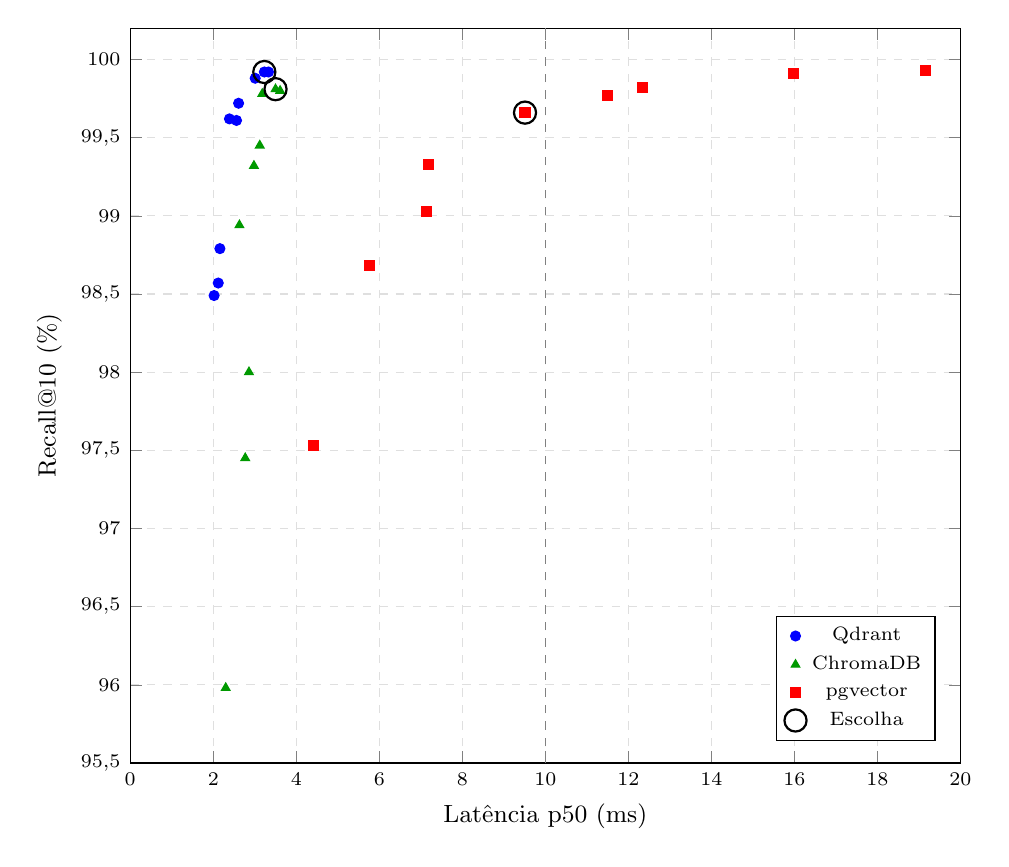
\begin{tikzpicture}
\begin{axis}[
    width=\textwidth, height=0.9\textwidth,
    xlabel={Latência p50 (ms)}, ylabel={Recall@10 (\%)},
    xmin=0, xmax=20, ymin=95.5, ymax=100.2,
    /pgf/number format/use comma,
    grid=major, grid style={dashed, gray!25},
    legend style={at={(0.97,0.03)}, anchor=south east, font=\scriptsize},
    tick label style={font=\scriptsize}, label style={font=\small}
]
\draw[gray, dashed] (axis cs:10,95.5) -- (axis cs:10,100.2);
\addplot[only marks, color=blue, mark=*, mark size=1.8pt] coordinates {(2.02,98.49) (2.39,99.62) (3.01,99.88) (2.12,98.57) (2.56,99.61) (3.23,99.92) (2.16,98.79) (2.61,99.72) (3.33,99.92)};
\addlegendentry{Qdrant}
\addplot[only marks, color=green!60!black, mark=triangle*, mark size=1.8pt] coordinates {(2.30,95.98) (2.63,98.94) (3.18,99.78) (2.77,97.45) (2.98,99.32) (3.50,99.81) (2.86,98.00) (3.12,99.45) (3.61,99.80)};
\addlegendentry{ChromaDB}
\addplot[only marks, color=red, mark=square*, mark size=1.8pt] coordinates {(4.41,97.53) (7.18,99.33) (12.33,99.82) (5.76,98.68) (9.51,99.66) (15.98,99.91) (7.13,99.03) (11.49,99.77) (19.16,99.93)};
\addlegendentry{pgvector}
\addplot[only marks, mark=o, mark size=4pt, black, thick] coordinates {(3.23,99.92) (3.50,99.81) (9.51,99.66)};
\addlegendentry{Escolha}
\end{axis}
\end{tikzpicture}
\caption*{(a) Métrica L2}
\end{minipage}%
\hfill
\begin{minipage}{0.49\textwidth}
\centering
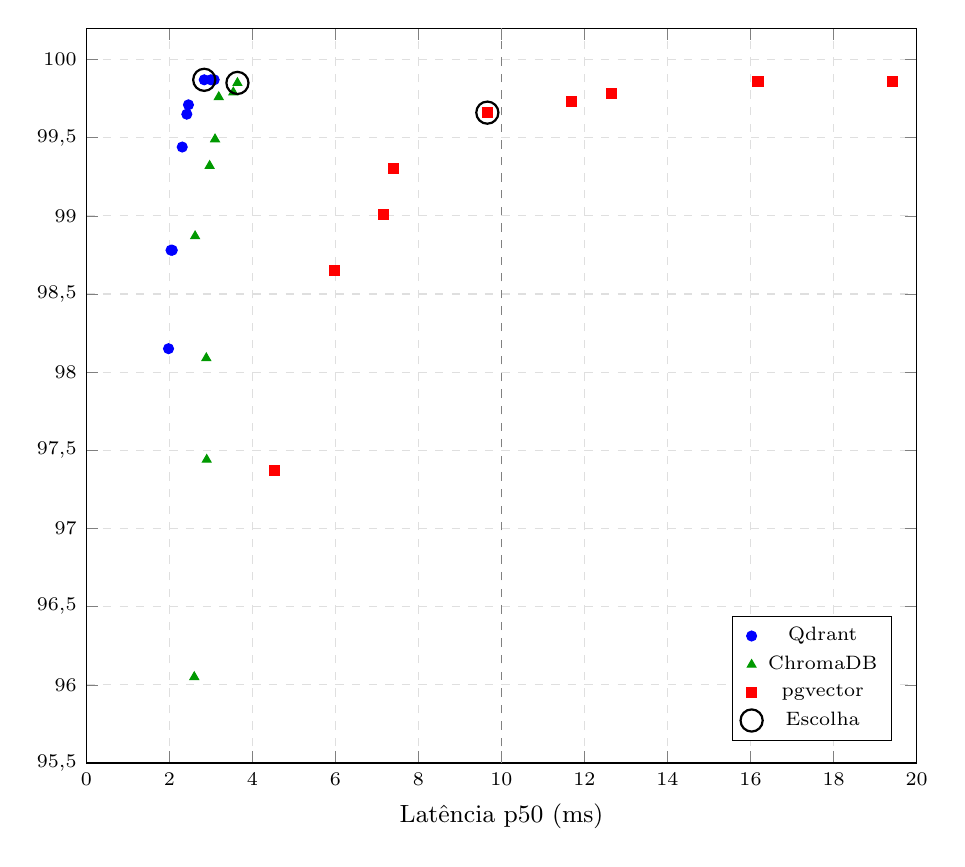
\begin{tikzpicture}
\begin{axis}[
    width=\textwidth, height=0.9\textwidth,
    xlabel={Latência p50 (ms)}, ylabel={},
    xmin=0, xmax=20, ymin=95.5, ymax=100.2,
    /pgf/number format/use comma,
    grid=major, grid style={dashed, gray!25},
    legend style={at={(0.97,0.03)}, anchor=south east, font=\scriptsize},
    tick label style={font=\scriptsize}, label style={font=\small}
]
\draw[gray, dashed] (axis cs:10,95.5) -- (axis cs:10,100.2);
\addplot[only marks, color=blue, mark=*, mark size=1.8pt] coordinates {(1.98,98.15) (2.31,99.44) (2.84,99.87) (2.04,98.78) (2.42,99.65) (3.00,99.87) (2.07,98.78) (2.46,99.71) (3.08,99.87)};
\addlegendentry{Qdrant}
\addplot[only marks, color=green!60!black, mark=triangle*, mark size=1.8pt] coordinates {(2.60,96.05) (2.62,98.87) (3.19,99.76) (2.90,97.44) (2.97,99.32) (3.54,99.79) (2.89,98.09) (3.10,99.49) (3.64,99.85)};
\addlegendentry{ChromaDB}
\addplot[only marks, color=red, mark=square*, mark size=1.8pt] coordinates {(4.54,97.37) (7.40,99.30) (12.64,99.78) (5.97,98.65) (9.66,99.66) (16.18,99.86) (7.16,99.01) (11.68,99.73) (19.42,99.86)};
\addlegendentry{pgvector}
\addplot[only marks, mark=o, mark size=4pt, black, thick] coordinates {(2.84,99.87) (3.64,99.85) (9.66,99.66)};
\addlegendentry{Escolha}
\end{axis}
\end{tikzpicture}
\caption*{(b) Similaridade de Cosseno}
\end{minipage}
\caption{Compromisso entre \textit{Recall@10} e latência mediana nas nove configurações de cada motor. Os círculos assinalam a configuração escolhida pelo critério; a linha tracejada marca o limiar de \SI{10}{\milli\second}.}
\label{fig:pareto_otimizacao}
\end{figure}
